%\FILE{usecase/hvac.tex}
\subsection{Use Case: HVAC Recommendation}

\paragraph*{Background.}
Heating, ventilation and air conditioning (HVAC) systems control air temperatures inside residential, commercial, and industrial  buildings. 
Desired room temperatures can be predetermined [/ fixed] by a technician, or regulated at any time by the user, through the use of a local thermostat, where the user chooses temperature setpoints. This manner of  HVAC control only considered user preference inputs at the moment the thermostat is programmed. Modern thermostats are capable of applying machine learning to leverage historical data on user preferences, and existing periodic variances in energy / electricity prices. To improve the HVAC system efficiency over time, introduction of other criterion / inputs into temperature setpoint decision making can reduce costs for consumers and in a scenario involving a million systems / units, present a potential for electricity service providers to better account for fluctuating consumer demand; and balance load. Here we are also including weather forecasts to the list of external inputs / or integrating weather research forecast WRF and we develop an algorithm that can calculate the optimal schedule of HVAC control. 

The algorithm deployment is on the cloud as a service, and every time it makes a new setpoint decision, the command is sent to the local thermostat (see Figure \ref{fig:hvac_general}). Various service frequencies were used to establish the proper pipeline for this application use case. This work aims to analyze the scalability and adaptability of such service scenarios and identify best practices that promote reusable implementations to support aspects of similar use cases addressed by them.

\begin{figure}[htb]
%\centering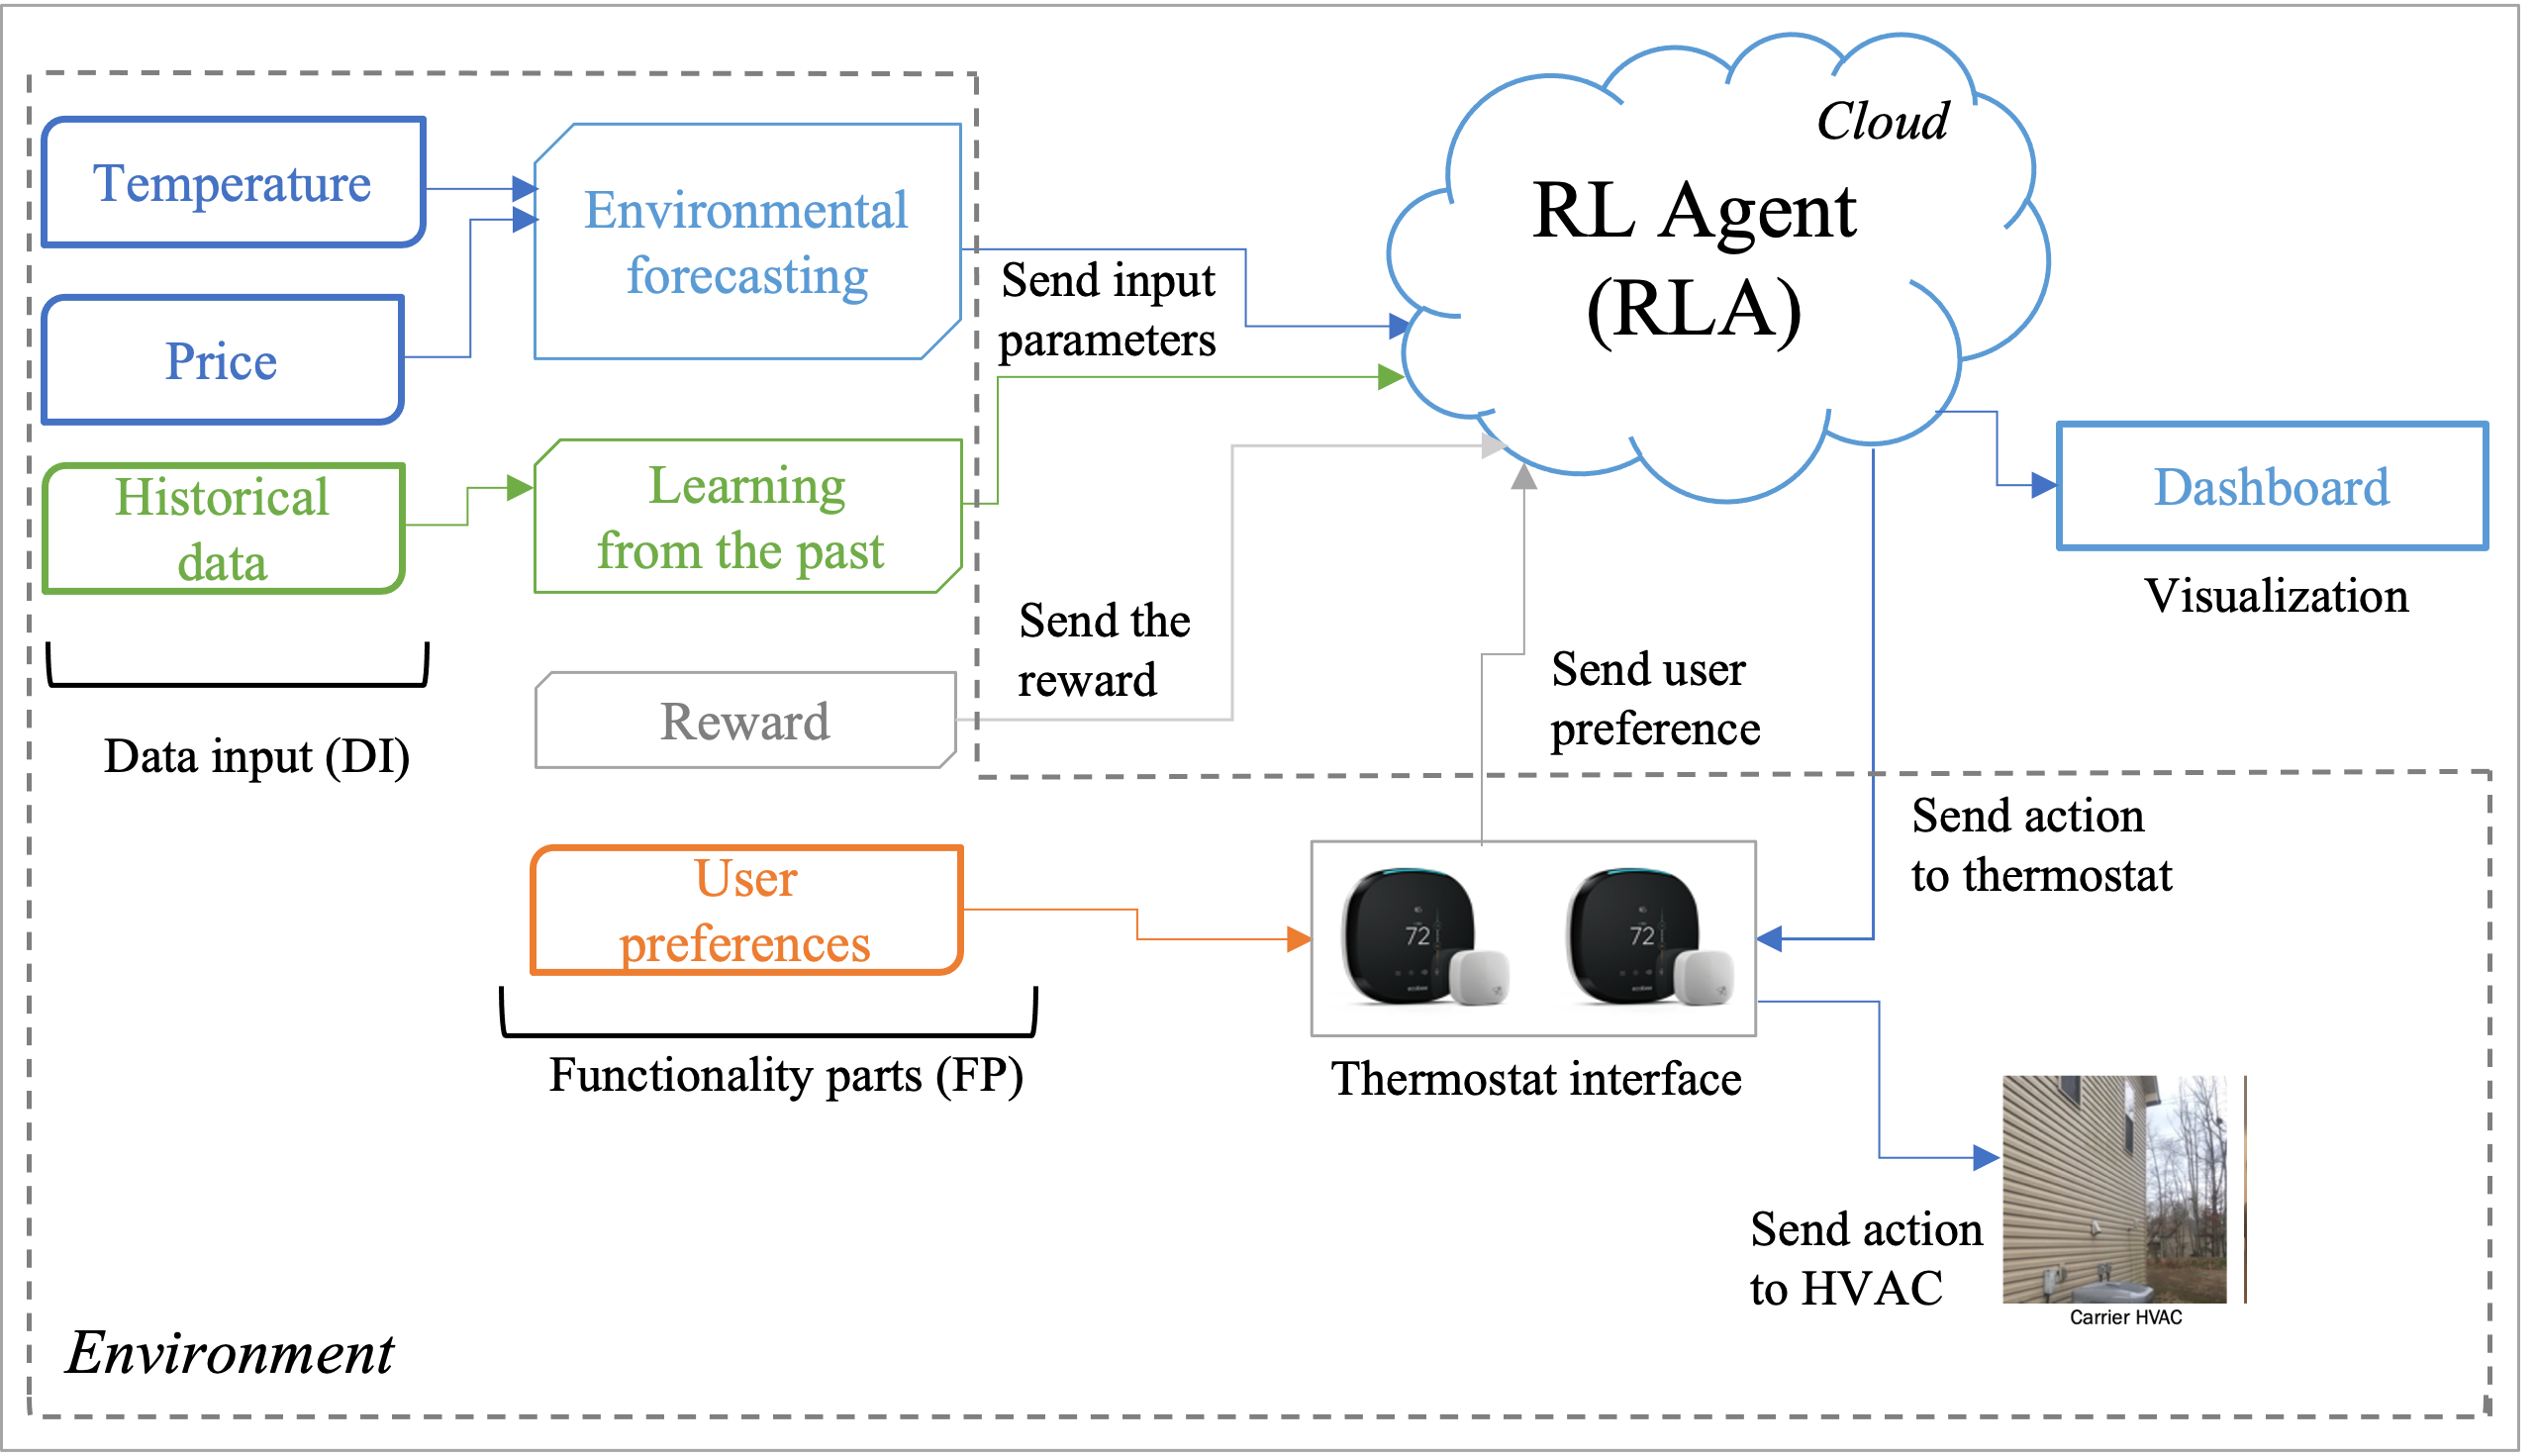
\includegraphics[width=1.0\columnwidth]{usecase/images/hvac-new-arch.png}
\centering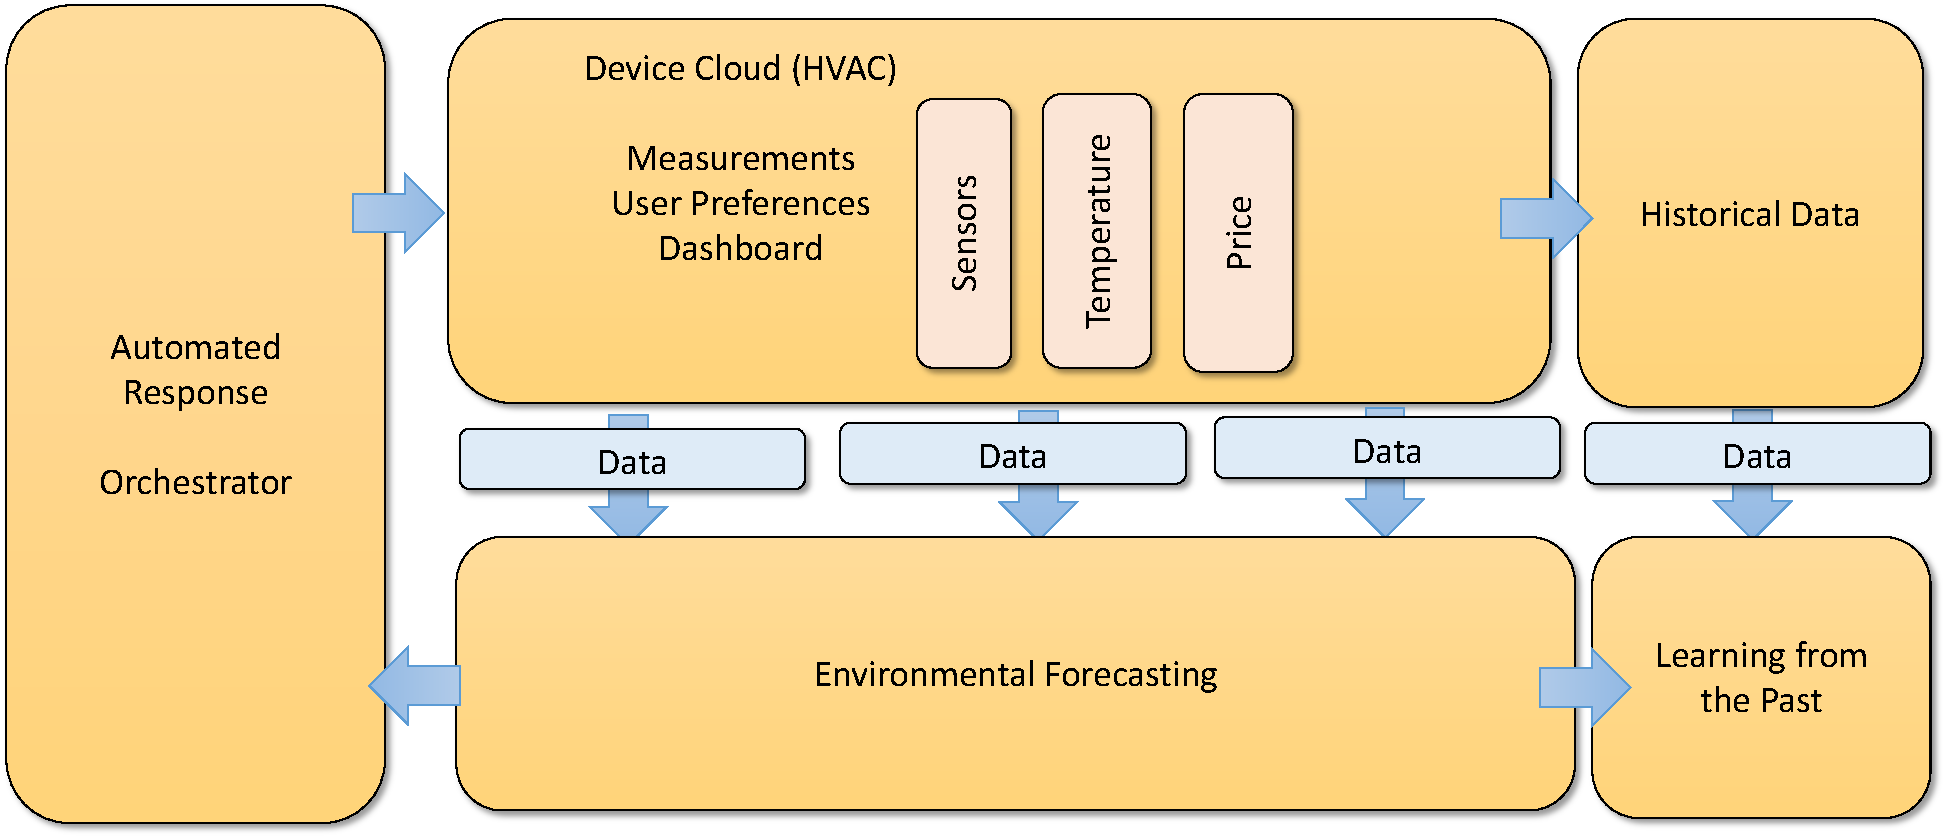
\includegraphics[width=1.0\columnwidth]{usecase/images/nist-hvac-layer.pdf}
\caption{General view of HVAC-to-Cloud system}
\label{fig:hvac_general}
\end{figure}

\paragraph*{System model.}
User comfort level is defined as the allowed temperature range in the house, the range can remain constant during the entire 24 hour cycle, or it can vary based on the time of the day or the day of the week. Since the temperature in the house is affected by the outdoor temperature our goal is to keep the internal temperature within the desired user comfort level. 
Energy prices fluctuate through out the day, driven by market dynamics. We describe the pricing function as a sequence of values $Price = {P_{t_1}, P_{t_2}, . . . , P_{t_m}}$ where $P_{t_i}$ corresponds to the price at time slot ${t_i}$. At each time slot, the service provider determines the electricity price and charges the customer at the given rate. We determine the user cost based on the price and energy consumption during the time slot. At time $t_{k-1}$, we observe the set of all variables of the system which includes information about the outdoor temperature, the indoor temperature, and the pricing. Based on all this information, the  algorithm makes a dynamic decision to set the HVAC set point. This represents the HVAC state in the next time-interval $t_k$. After executing the HVAC setpoint action, we observe the system during time step $t_k$. These steps are executed in periodic intervals, as presented in Figure \ref{fig:hvac_general} and the setpoint recommendation process require advanced machine learning algorithm (e.g, reinforcement learning) \cite{kotevska2020rl}. %Accurate recommendations can save energy and reduce cost \TODO{3rd time mentioned}. 


We organized this functionality in three parts: Data input (DI), Functionality parts (FP), and RL agent (RLA). DI collects the data needed for the calculation, such as the following: %weather temperature, price, and historical data. 
\begin{itemize}
    \item Temperature -- Collects current weather temperature.
    \item Price -- Collects current electricity price.
    \item Historical data -- Extract needed data fields and packs it into an intermediate file format. Input data from the output of temperature and price.
\end{itemize}

%FP learns from the past and makes environmental forecasting, such as the following: 
FP prepares the inputs for RLA, they are the following:
\begin{itemize}
%\item hist -- Prepares history data points and creates initial condition weights.
    \item Learning from the past -- Learns from previous user and system activities.
    \item Environment forecasting -- Incorporates future price and temperature forecasting for timestamp ${t_{i+1}}$.
    \item Reward -- Generates reward based on the current temperature, price, and user input.
    \item User preferences -- Creates rules based on user temperature preferences.
\end{itemize}

RLA model estimates the next set-point ${t_{i+1}}$ using the inputs from FP, such as: 
\begin{itemize}
    \item RL agent --  Interpolates the output from DI, FP, reward, and user preferences and generates action recommendation for the temperature.
\end{itemize}

Figure \ref{fig:hvac_general} shows the general modeling system flow chart. 

%\begin{figure}[htb]
%\centering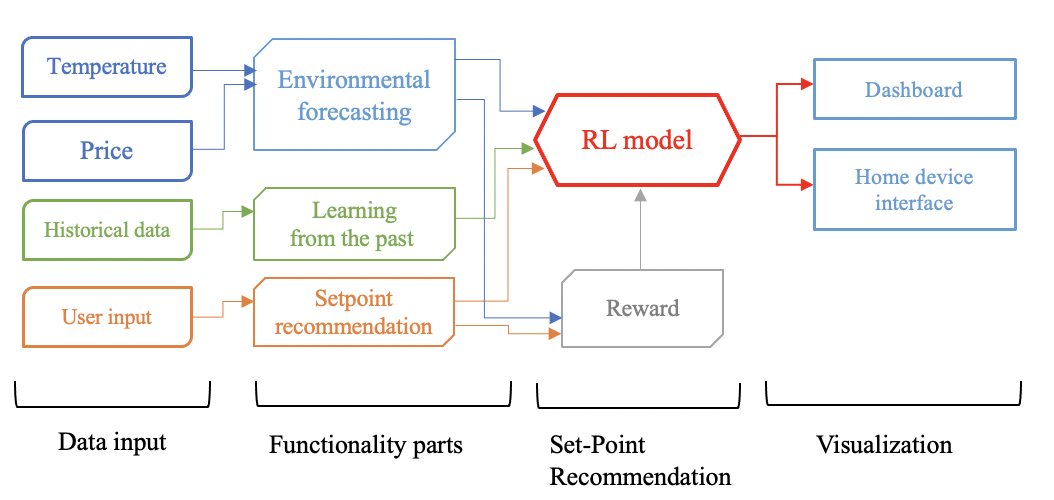
\includegraphics[width=1.0\columnwidth]{usecase/hvac_flowchart.png}
%\caption{HVAC general modeling system flow chat.}
%\label{fig:hvac_flowchart}
%\end{figure}

% \paragraph*{Functionalities and Activities} (based on Big Data Application Provider of NBDIF Ref. Architecture).

%In this case study, we only focus on three main functionalities, namely EF, LP and SPR, and their activities. Figure \ref{fig:hvac_func_diagram} shows the cross-functional diagram for their actions TODO{plan to remove fig 4}.


%\begin{figure}[htb]
%\centering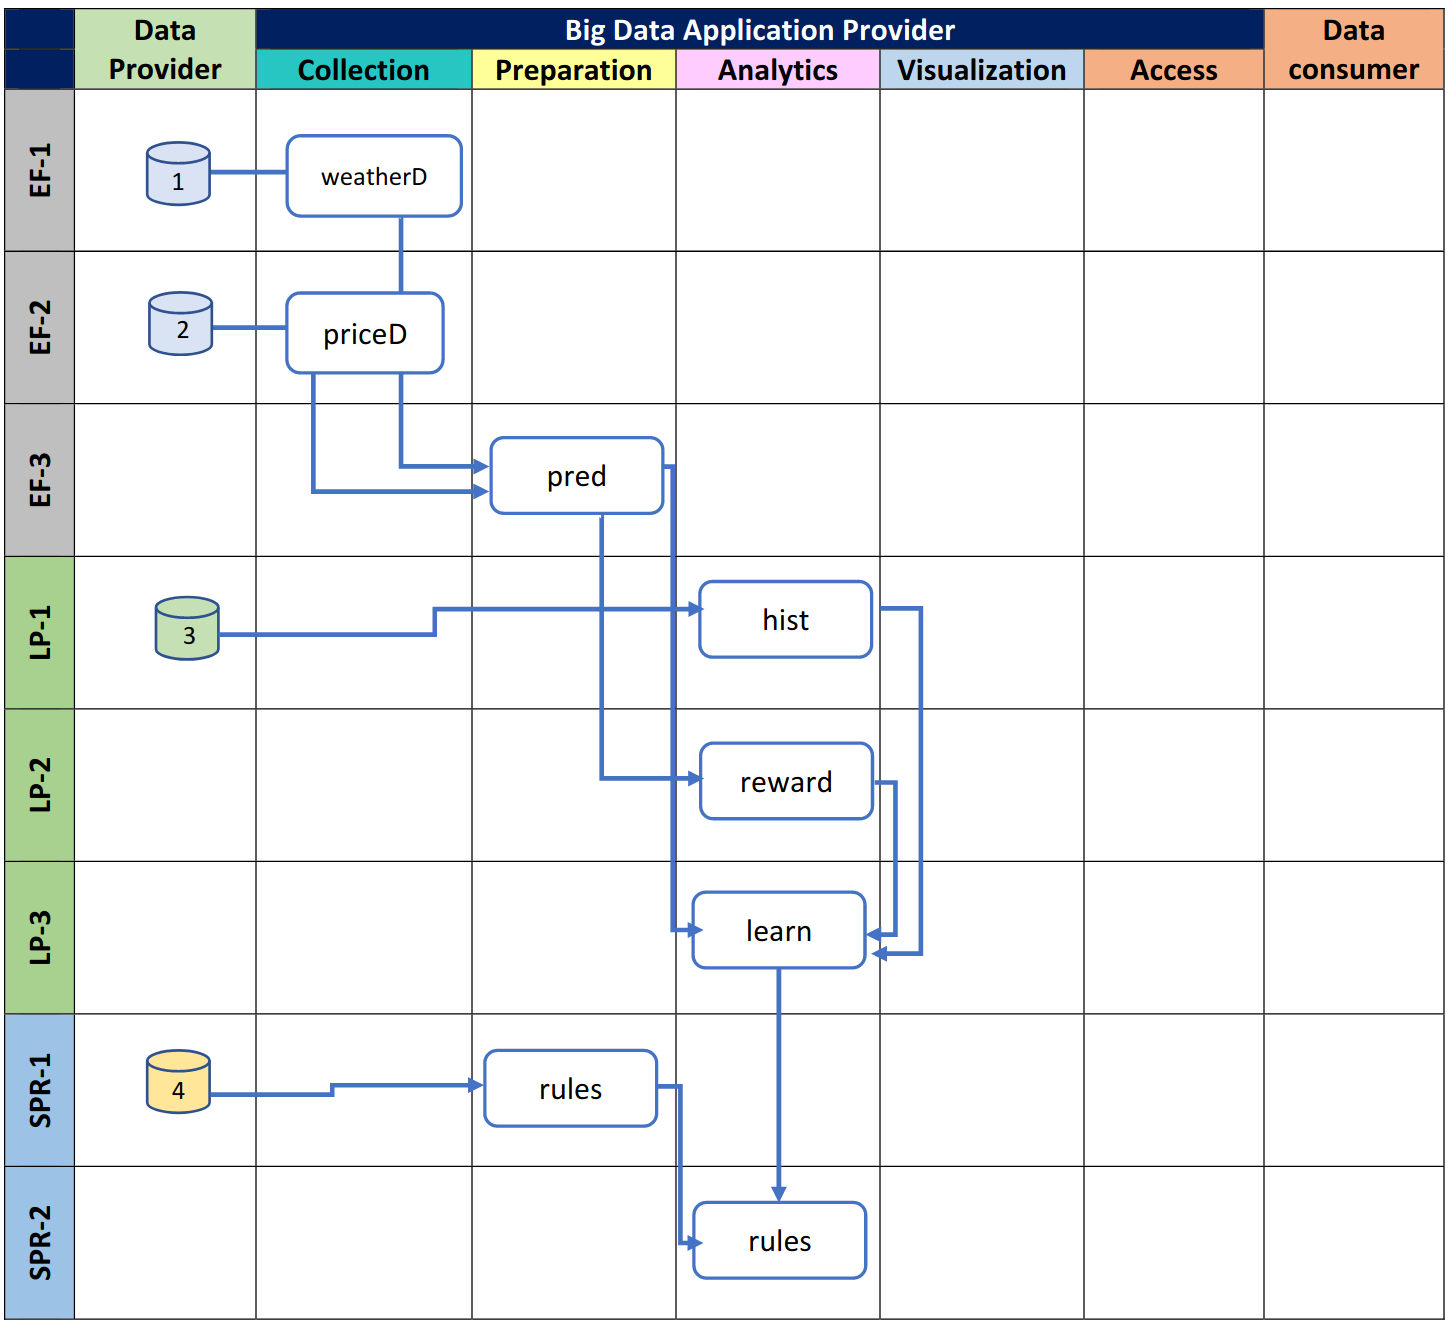
\includegraphics[width=1.0\columnwidth]{usecase/hvac_functional.png}
%caption{Cross-Functional Diagram HVAC Recommendation.}
%\label{fig:hvac_func_diagram}
%\end{figure}

%\TODO{evaluate this section}

%FP Activities:
%RLA Activities:

Reward is a function of temperature violation and cost. This function is specific to the algorithm that was used in this case reinforcement learning (RL). If the temperature is above the desired setpoint and energy cost is high the reward is negative. While if the temperature is within the setpoint range and the energy price is low the reward is positive. This allows the RL-based method to learn the optimal behavior through continuous interaction with a building environment and without referring to any prior model knowledge. 

The results are presented on the home device interface and historic results are presented on the dashboard using the cloud-as-a-service option.

This setup is a general setup that is applicable to one-zone models. Results have shown that RL model has high generalization and adaptability to unseen environments, which indicates its practicability for real-world implementation \cite{du2021intelligent}. The same functionality can be used with different building models and retail price models \cite{du2021intelligent}. 

%\paragraph*{Algorithm}

%\TODO{No datasets provided.}

This use case has the implicit requirements needing the following aspects to be addressed by the framework we develop.

\begin{enumerate}

\item{\bf AS vendor neutral cloud and computer service integration.} 

\begin{enumerate}
  \item {\bf AS in cloud.} The Analytics Services are on the cloud, and the user has Vendor Neural Access Interface to monitor the current and past behavior. The users can also manage their preferred HVAC behavior using the provided interface by the command line.
  \item {\bf AS in LCCF.} This feature does not apply to the current use case. However an extension could be adressing larger scales of the application while integrating analysis on a much larger scale.
  \item {\bf AS in microservices.} This feature does not apply to this use case. We anticipate that future services may use microservices in order to increase portability.
\end{enumerate}

\item{\bf AS architecture.} 

\begin{enumerate}
  \item{\bf AS vendor neutral interfaces.} The user has access to two interfaces: a) a web-based dashboard to monitor the current and past HVAC status changes and indoor temperature; b) an HVAC embedded home interface where the user can check and change the desired indoor temperature.
  \item{\bf AS REST.} The HVAC home interface accepts user preferences and sends them to the cloud using REST services. 
  \item{\bf AS layers such as interface, service layer, and provider layer.} The vendor uses Privacy Cloud for the calculations and data storage, Analytics Services for decision-making analysis, Cooperation Service for external data inputs, and Command line for the user to send requests and make any service adjustments.
\end{enumerate}

\item{\bf AS workflow.} 

\begin{enumerate}
  \item{\bf AS catalog and registry.} For this use case, the catalog of services only supports a few operations they are i) temperature set-point adjustment based on outdoor temperature, price, user schedule, and preferences; ii) historical overview; iii) receiving user input for set-point adjustment.
  \item{\bf AS cooperation.} The cooperation is with external services used for decision-making analysis (e.g., weather forecast, utility energy price).
  \item{\bf Competition.} This feature does not apply to this use case. In future alternative analysis algorithms could be integrated that allow collaborative results but also competition.
  \item{\bf AS orchestrator.} This feature does not apply to this use case. However an extension could be envisioned that allows the execution of the analysis on different geographically distributed resources to circumvent outages of the center due to unforeseen challenges, such as extreme weather events or power outages.
\end{enumerate}


\item{\bf AS calculation.}

\begin{enumerate}
  \item{\bf AS with DL.} In this case is used DL ( e.g., reinforcement learning (RL)) for the decision-making analysis.
  \item{\bf AS data analytics.} In this use case, data analytics provides visualization and statistics for the past behavior and decision-making recommendations for HVAC setpoint settings.
\end{enumerate}

\item{\bf AS security.} The data transfer to and from the cloud is over a secure protocol. 


\end{enumerate}


